\chapter{實驗與執行結果}
%\label{c:intro}
本章利用上一章所介紹的數據擷取方法,在實際的解答平台雛形上,進行數據的即時採集、畫面監控與模擬作答影片;
另外也利用上一章所介紹的數據分析方法,針對實際的數據進行基礎的分析。以下分別說明。
\section{網頁平台數據監測}
\subsubsection{顯示頁面}
在網頁的平台只有觀察使用者打字與紀錄時間並畫圖顯示。(圖4.1)為網頁偵測的頁面,中間的空白處就是給使用者打字的地方,並且在進行打字同時計算字數回傳,進而畫出時間字數的折線圖。
	\begin{figure}[H] 
	\centering 
	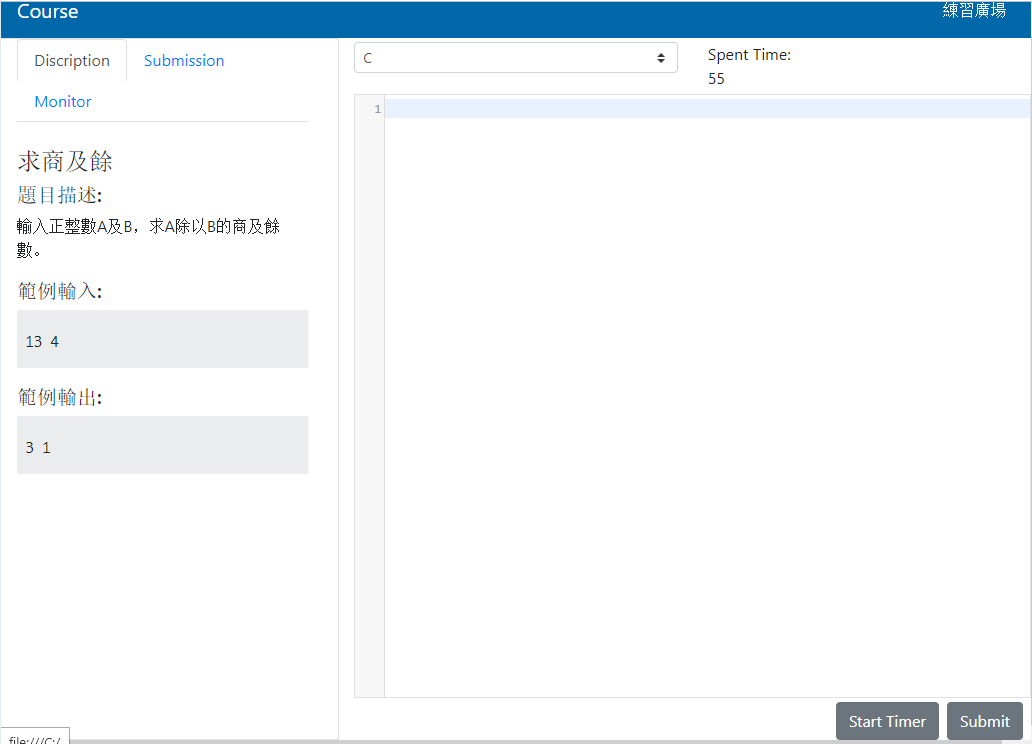
\includegraphics[width=0.7\textwidth]{web_part.png} 
	\caption{網頁顯示頁面} 
	\label{Fig.4.1} 
	\end{figure}

\subsubsection{網頁的圖形輸出}
首先觀察從作答畫面所抓到的數據資料與圖形的顯示。圖4.2是針對一個簡單的範例題,
在作答過程中所擷取的資料和圖形畫面結果:
\begin{enumerate}[1.]
	\item 簡短程式碼(圖4.2)\\
	左邊為實際作答的網頁畫面,右邊則是即時監測的圖形數據。在右邊的畫面中可以看到累計字數有上升或下降的情形,這表示使用者在撰寫程式時,使用了backspace倒退鍵或刪除鍵進行程式的修改。
	\begin{figure}[H] 
		\centering 
		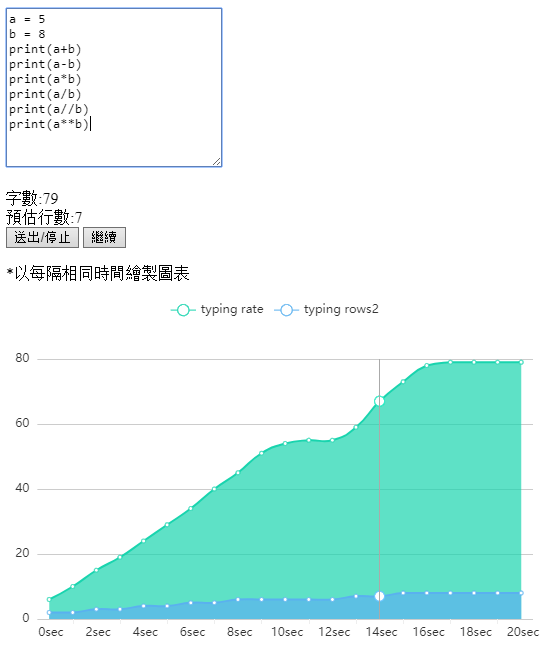
\includegraphics[width=0.7\textwidth]{4_2.png} 
		\caption{簡短程式碼輸出} 
		\label{Fig.4.2} 
	\end{figure}
	\item console的訊息(圖4.3)\\
	除了輸出的統計圖形,我們也可以使用console觀察系統擷取數據的過程,可以看到每當網頁介面的數據有所變化時,監控畫面會把數據顯示在圖形與網頁上。這裡可以看到資料每隔3秒鐘擷取一次,這個擷取的時間間隔必須合理的設定,如果間隔太短,固然可以得到更密集的資料,但是可能會造成太多冗餘的資料,以及資料太過龐大的問題,也會增加分析的複雜度;但如果設定太長,可能會漏失一些重要的資訊。此處設定為3秒鐘取一次。
	\begin{figure}[H] 
		\centering 
		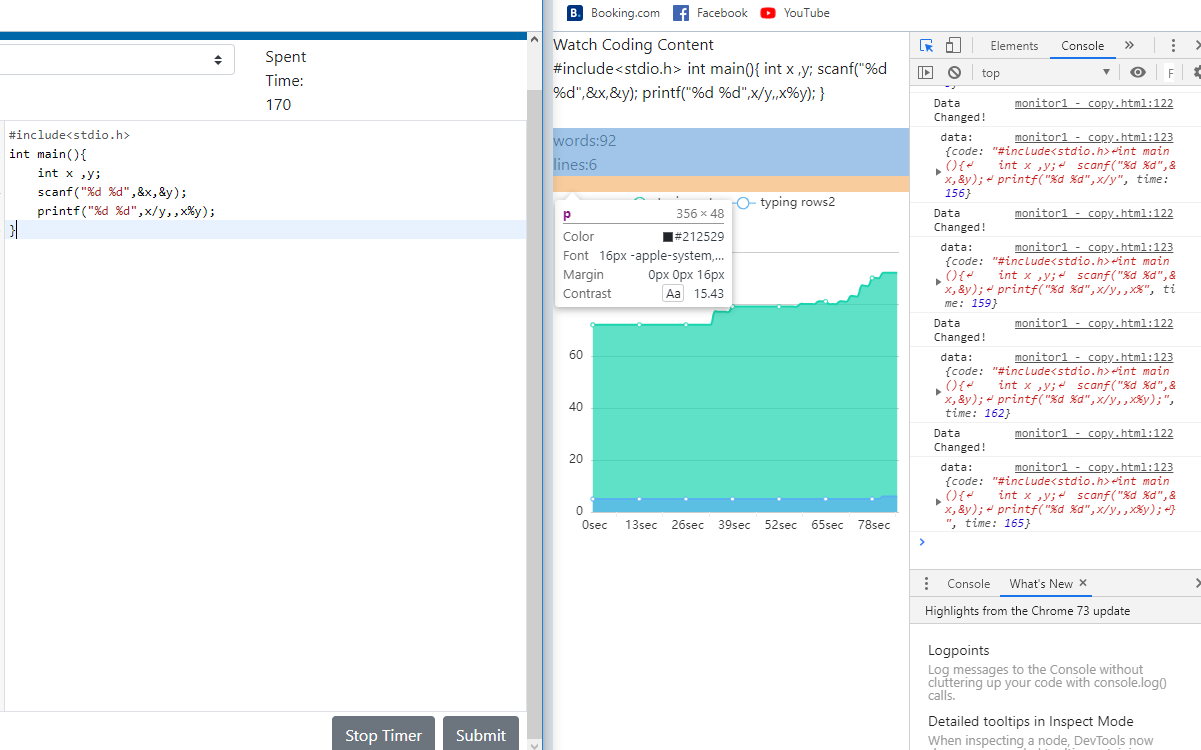
\includegraphics[width=0.7\textwidth]{4_3.png} 
		\caption{console的訊息} 
		\label{Fig.4.3} 
	\end{figure}
	\item 複製貼上(圖4.4)\\
	若是使用者貼上大量文字的話,圖形變化會成階梯狀,主要因數據變化的幅度比自然打字大很多的緣故。透過統計畫面的顯示,可以估測使用者在此用了複製貼上的動作。
	\begin{figure}[H] 
		\centering 
		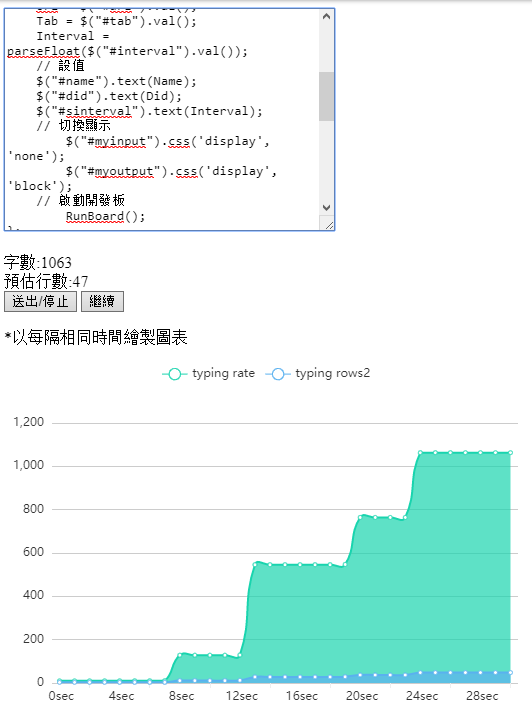
\includegraphics[width=0.7\textwidth]{4_4.png} 
		\caption{複製貼上的輸出} 
		\label{Fig.4.4} 
	\end{figure}
\end{enumerate}

\subsubsection{模擬作答畫面}
除了觀察使用者作答的統計資訊之外,我們也可以利用擷取的取樣資料,模擬同學作答的畫面,也可以產出模擬作答的影片。\\
\begin{itemize}
	\item 模擬作答畫面的運作:\\
	打開模擬作答畫面,一開始會是一個空白的框(圖4.5)
		\begin{figure}[H] 
		\centering 
		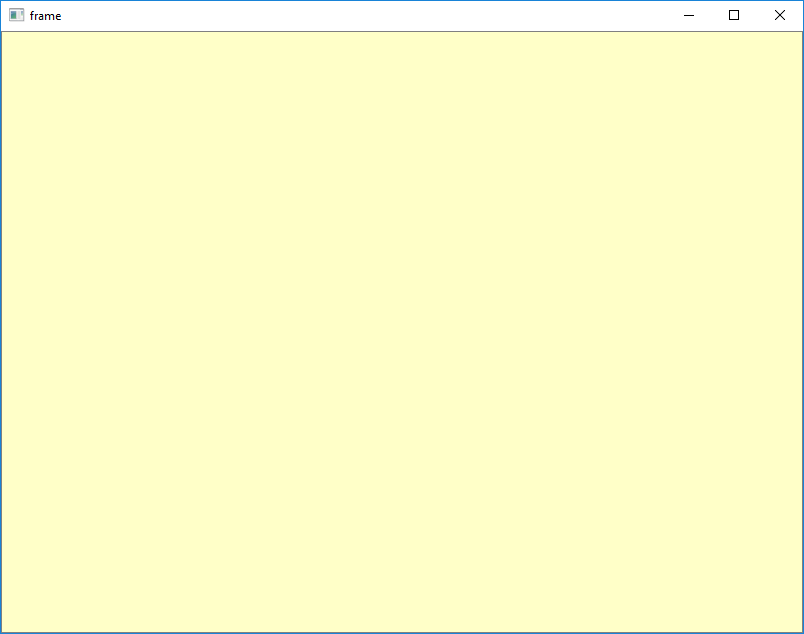
\includegraphics[width=0.7\textwidth]{video_space.png} 
		\caption{模擬作答啟始畫面} 
		\label{Fig.4.4.1} 
		\end{figure}
	當使用者在作答介面進行打字的時候,模擬畫面的內容也會開始改變。前面提過Firebase資料庫可以自動通知程式資料有更新的事件,我們利用更新的數據來進行模擬畫面的更新動作。這樣一來,當使用者在打字的時候,模擬畫面也會在很小的延遲時間下同步更新。(圖4.6)
	\begin{figure}[H] 
		\centering 
		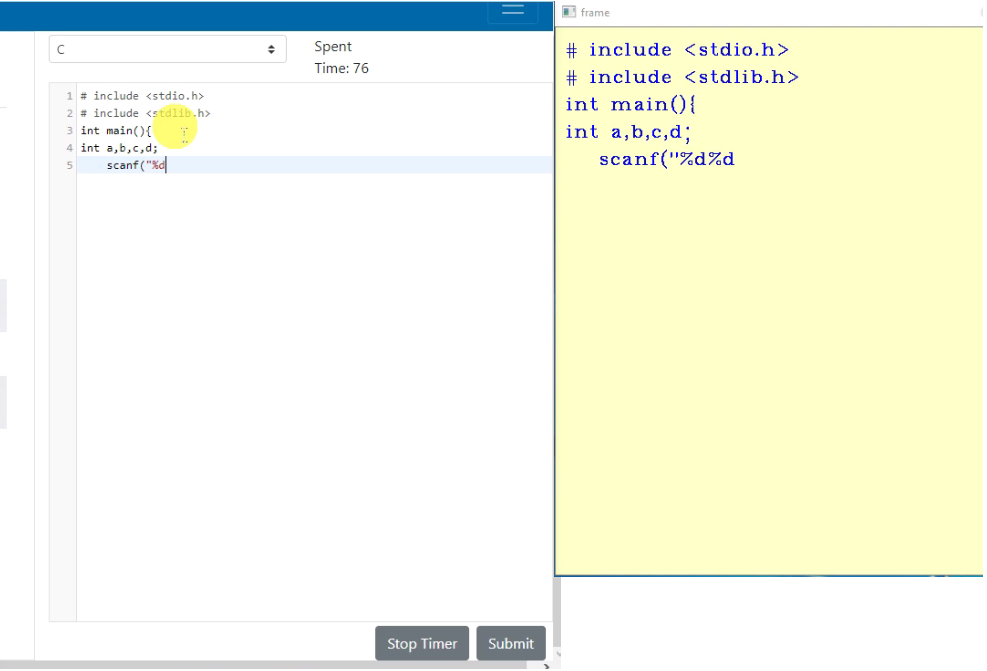
\includegraphics[width=0.7\textwidth]{frame.png} 
		\caption{模擬作答的過程畫面} 
		\label{Fig.4.4.2} 
	\end{figure}

	當監控結束之後,可以把這些模擬的畫面輸出成影片,存成一個AVI影片檔。
	
	\item 影片動作與實際動作:\\
	模擬作答的錄製影片,因為有少量的時間延遲,以及資料取樣的問題,在此想把輸出的AVI影片檔與真正打字的影片檔拿來做一比較,
	於是在打字的時候使用螢幕錄影軟體進行錄製,並拿來與模擬的錄製畫面相比,結果如圖4.7所示。\\
			\begin{figure}[H] 
		\centering 
		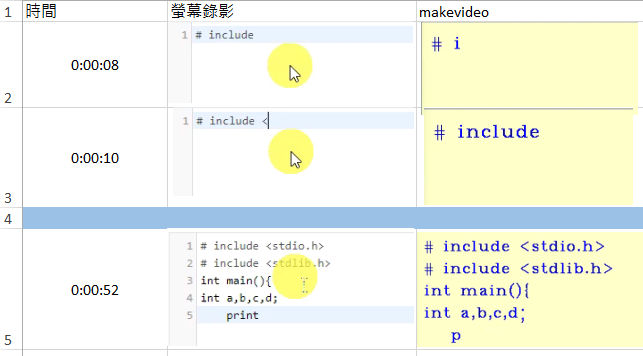
\includegraphics[width=0.7\textwidth]{diff.png}
		\caption{螢幕錄影與makevideo比較} 
		\label{Fig.4.4.3} 
		\end{figure}
	可以看出影片的動作會慢於實際的打字速度,因為在取值時有設定固定的秒數,因此若是使用者不間斷的打字必然不能完整呈現,所以模擬畫面所產生的輸出影片與實際上螢幕錄影的影片有少許延遲,但大體上已經可以接近真實的模擬使用者在打字時的種種動作。另外,我們用來製作模擬作答影片的資料,主要是取樣的文字資料,其資料量比實際在螢幕錄製的影片要少得多,這樣比較容易做到即時的處理。

	\item 資料的後續處理:\\
	在第三章的基礎數據分析中,我們使用Python程式做了一些統計分析,那時候採用的數據是模擬產生的。那有了實際平台測試的樣本資料之後,我們也可以拿這些實際的資料來進行分析。因此我們也撰寫了一個Python程式,同樣經由Firebase把使用者的作答取樣資料抓取下來,供作後面的統計分析。抓取的取樣資料如圖4.8所示。
	\begin{figure}[H] 
		\centering 
		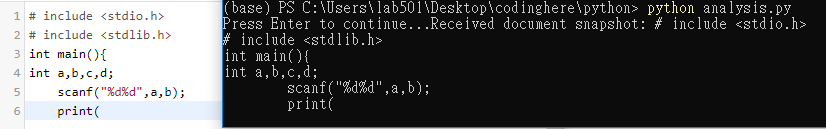
\includegraphics[width=0.7\textwidth]{anysis.png}
		\caption{python抓下的文字} 
		\label{Fig.4.4.4} 
	\end{figure}
\end{itemize}

\section{數據的統計分析}
\vspace*{-4mm}
我們利用上一章所說明的Python程式碼在擷取的實驗數據上進行分析,此處分別使用了10組與30組的數據資料。
\subsubsection{個別的圖形與數據}
每一組數據會產生如圖4.9的一組圖形,以下只列每次產生的數據最基本的折線圖,共10組。(圖4.10)
	\begin{figure}[H] 
	\centering 
	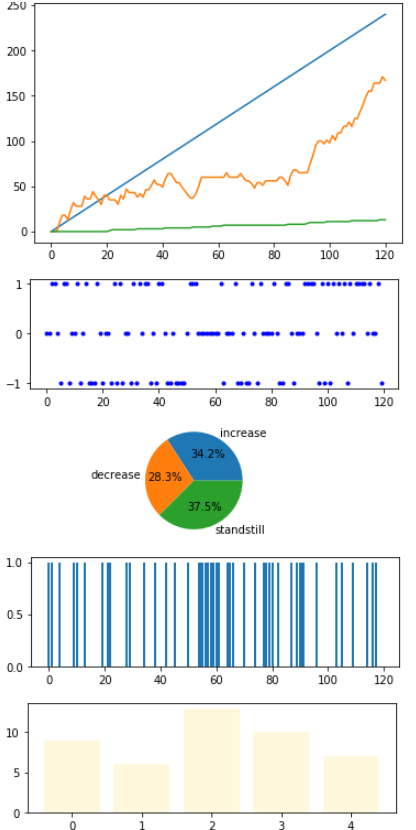
\includegraphics[width=0.5\textwidth]{4_5.png} 
	\caption{圖形組} 
	\label{Fig.4.5} 
	\end{figure}
	\begin{figure}[H] 
	\centering 
	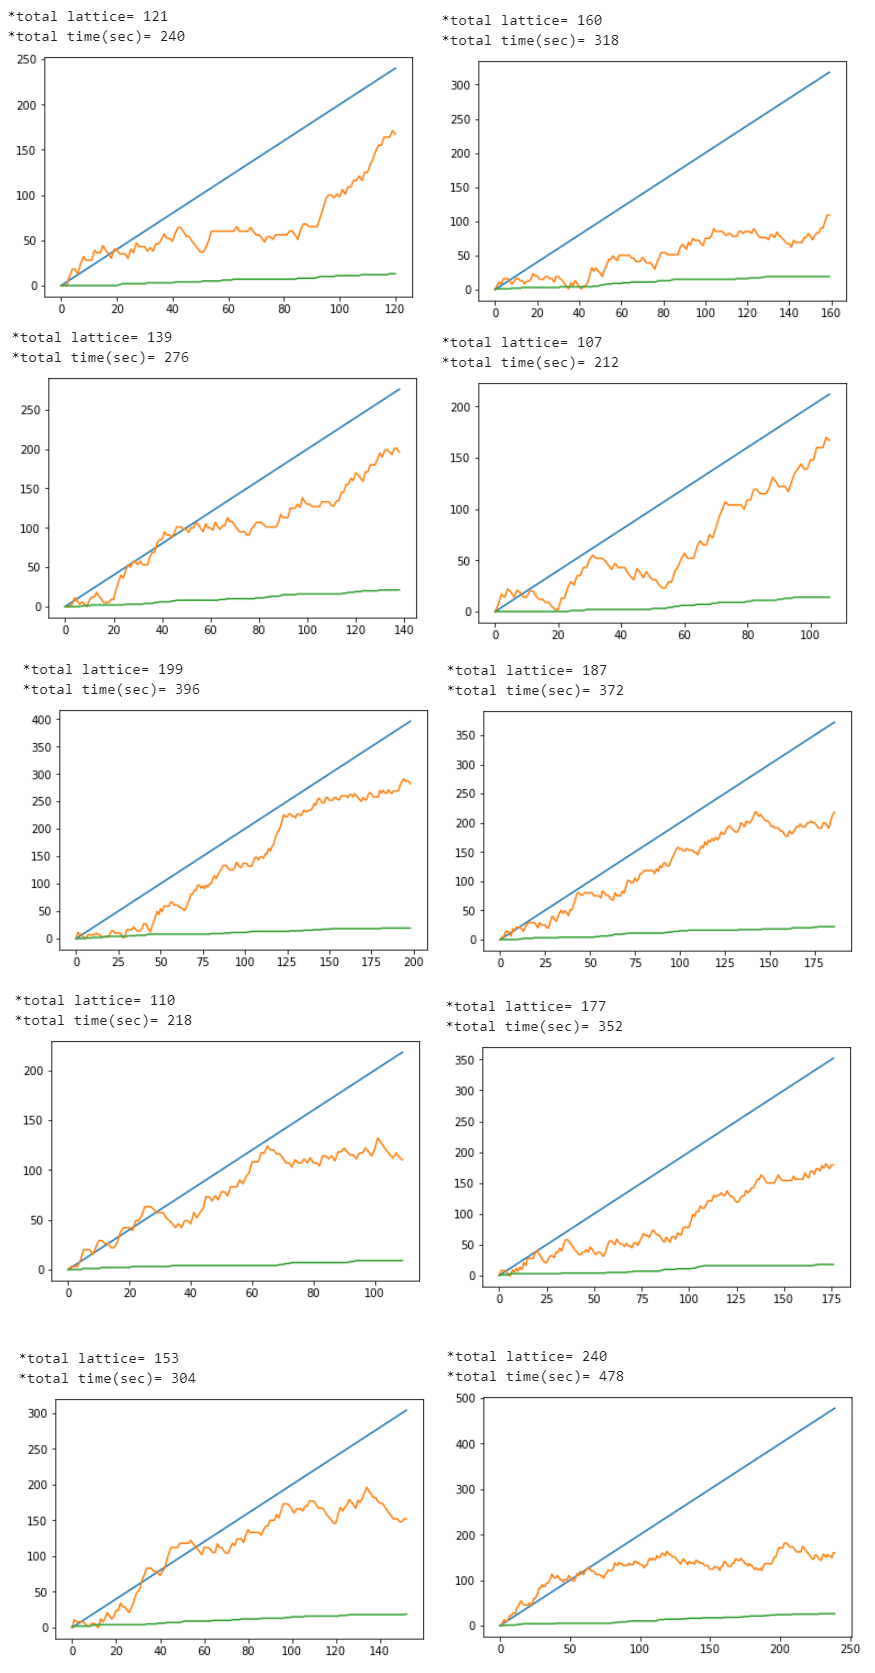
\includegraphics[width=0.7\textwidth]{4_6.png} 
	\caption{10組折線圖} 
	\label{Fig.4.6} 
	\end{figure}

\subsubsection{統整的表格數據}
把全部的數據統整起來製程表格,表格一樣使用Python,可以直接在Colab上輸出顯示結果。\\
1. 10組結果(圖4.11)
	\begin{figure}[H] 
	\centering 
	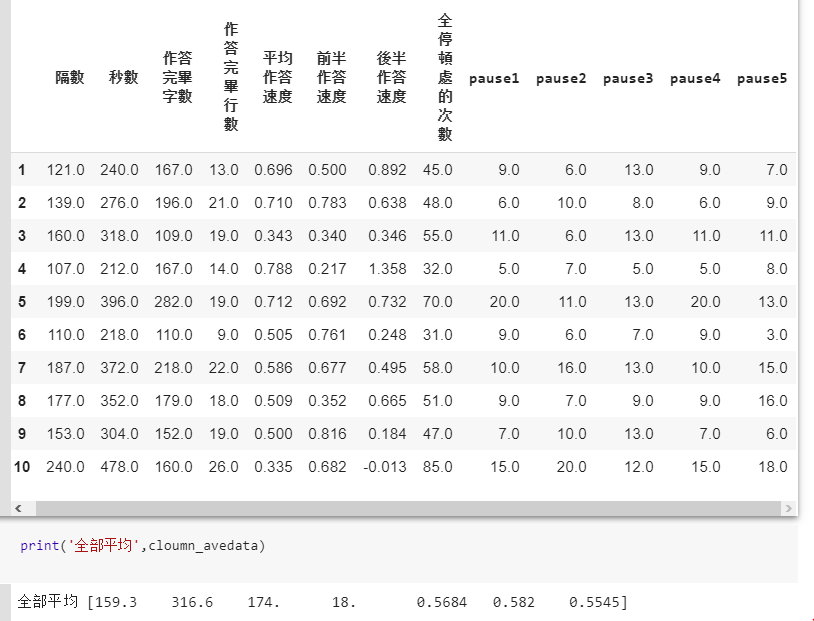
\includegraphics[width=0.7\textwidth]{4_7.png} 
	\caption{10組結果表格圖} 
	\label{Fig.4.7} 
	\end{figure}

\newpage
2. 30組結果,因資料較龐大所以使用表格顯示(表4.1))\\
\begin{table}[]
	\label{table1}
	\begin{tabular}{lllllllll}
		& 隔數  & 秒數  & 作答完畢字數 & 作答完畢行數 & 平均作答速度 & 前半作答速度 & 後半作答速度 & 全停頓處的次數 \\
		1  & 115 & 228 & 193    & 19     & 0.846  & 0.833  & 0.86   & 39      \\
		2  & 190 & 378 & 343    & 14     & 0.907  & 0.984  & 0.831  & 72      \\
		3  & 212 & 422 & 230    & 26     & 0.545  & 0.417  & 0.673  & 69      \\
		4  & 149 & 296 & 204    & 12     & 0.689  & 0.716  & 0.662  & 52      \\
		5  & 172 & 342 & 246    & 17     & 0.719  & 0.374  & 1.064  & 53      \\
		6  & 135 & 268 & 94     & 15     & 0.351  & 0.425  & 0.276  & 46      \\
		7  & 219 & 436 & 299    & 26     & 0.686  & 0.583  & 0.789  & 67      \\
		8  & 133 & 264 & 189    & 19     & 0.716  & 0.803  & 0.629  & 51      \\
		9  & 111 & 220 & 171    & 11     & 0.777  & 1.509  & 0.045  & 31      \\
		10 & 127 & 252 & 80     & 15     & 0.317  & 0.516  & 0.119  & 47      \\
		11 & 140 & 278 & 242    & 19     & 0.871  & 0.964  & 0.777  & 51      \\
		12 & 241 & 480 & 288    & 26     & 0.6    & 0.354  & 0.846  & 77      \\
		13 & 222 & 442 & 371    & 25     & 0.839  & 1.009  & 0.67   & 70      \\
		14 & 220 & 438 & 288    & 28     & 0.658  & 0.749  & 0.566  & 71      \\
		15 & 247 & 492 & 218    & 28     & 0.443  & 0.472  & 0.415  & 84      \\
		16 & 158 & 314 & 176    & 18     & 0.561  & 0.924  & 0.197  & 52      \\
		17 & 162 & 322 & 136    & 17     & 0.422  & 0.472  & 0.373  & 61      \\
		18 & 227 & 452 & 267    & 29     & 0.591  & 0.633  & 0.549  & 81      \\
		19 & 199 & 396 & 139    & 19     & 0.351  & 0.641  & 0.061  & 75      \\
		20 & 240 & 478 & 209    & 32     & 0.437  & 0.552  & 0.322  & 75      \\
		21 & 202 & 402 & 178    & 25     & 0.443  & 0.597  & 0.289  & 61      \\
		22 & 189 & 376 & 349    & 22     & 0.928  & 0.793  & 1.064  & 53      \\
		23 & 203 & 404 & 161    & 26     & 0.399  & 0.302  & 0.495  & 65      \\
		24 & 146 & 290 & 197    & 8      & 0.679  & 1.186  & 0.172  & 48      \\
		25 & 195 & 388 & 185    & 17     & 0.477  & 0.629  & 0.325  & 70      \\
		26 & 93  & 184 & 61     & 10     & 0.332  & 0.946  & -0.283 & 25      \\
		27 & 98  & 194 & 60     & 2      & 0.309  & 0.33   & 0.289  & 28      \\
		28 & 93  & 184 & 132    & 8      & 0.717  & 0.772  & 0.663  & 33      \\
		29 & 204 & 406 & 225    & 18     & 0.554  & 0.951  & 0.158  & 65      \\
		30 & 120 & 238 & 91     & 16     & 0.382  & 0      & 0.765  & 52     
	\end{tabular}
\caption{30組數據}
\end{table}

\newpage
\section{結果討論}
\subsection{數據即時監控部份}
\begin{itemize}
	\item 本研究藉由網頁前端及時偵測使用者的打字情況,並且計算其字數與花費時間。不同於其餘答題系統需要繳交後才知曉使用者的答題狀況,此方法因為其實時偵測的特性,使用者的答題習慣也可以藉由字數與時間看出端倪。
	\item 目前根據擷取的資料,只做了字數、行數與時間的統計圖表,如可以增加更多的鍵盤偵測將會使系統更加完善,這是未來可以持續改善的地方。
	\item 在影片輸出部分,本研究比較了經由透過擷取數據所產出的模擬作答畫面與影片錄製結果,雖輸出的影片不及真正的錄影資訊來的完整與細緻,但輸出的影片能明確抓取使用者在作答時進行的改動。
\end{itemize}
\subsection{數據分析部份}
\begin{itemize}
	\item 進行分析的部分最大的難處是缺少實際數據,因此在本論文在一開始研究的時候,先使用程式產生模擬數據,再以模擬數據撰寫及測試一些基本的分析方法,但模擬的數據理所當然地不及實際數據來的真實與客觀。本章則透過實際的作答平台採集實真實的數據進行分析,不過因為平台仍處於雛形階段,也沒有大量數據可以採集,因此只有基本的測試結果。
	\item 在討論數據停頓的密集程度的地方(圖3.16),目前選用的方法是把整體數據分成五個等分並寫計算每一等分的停頓次數;而此部分也是不夠嚴謹的,因可能密集的地方會被分組計算而分割,所以分區計算的方法並不能表示絕對的疏密程度。
\end{itemize}
